\documentclass[a4paper,twoside]{article}
\usepackage[T1]{fontenc}
\usepackage{graphicx}
\usepackage{calc}
\usepackage{amssymb}
\usepackage{amsmath}
\usepackage{pslatex}
\usepackage{apalike}
\usepackage{booktabs}
\usepackage{algorithm2e}
\usepackage[bottom]{footmisc}
\usepackage[hidelinks,breaklinks]{hyperref}
\usepackage{SCITEPRESS}
\hypersetup{pdftitle={Linking Candidate Coverage to Decision Quality: A Framework for LLM Planning Evaluation},pdfauthor={Alexander V. Mantzaris and James H. Korris},pdfsubject={ICAART 2027 camera-ready revision},pdfkeywords={LLM Planning, Semantic Validation, Evaluation},pdfcreator={LaTeX}}

\begin{document}
\title{Linking Candidate Coverage to Decision Quality: A Framework for LLM Planning Evaluation}
\author{\authorname{Alexander V. Mantzaris\sup{1} and James H. Korris\sup{2}}
\affiliation{\sup{1}Dr. Yvette Kanouff School of Data, Mathematical, and Statistical Sciences,\\
UCF, 4000 University Blvd, Orlando, FL, USA}
\affiliation{\sup{2}Creative Technologies Inc.}
\email{alexander.mantzaris@ucf.edu, james.korris@cretecinc.com}}
\keywords{LLM Planning, Semantic Validation, Candidate Coverage, Decision Correctness, Evaluation.}
\abstract{A traveler might ask a planning assistant for a journey arriving by a certain time with at most one transfer. A language model translates the request into machine checkable requirements that planning software uses to choose a journey. Confusing the arrival deadline with a departure deadline could produce a journey that passes those checks yet arrives late. An overall success rate cannot explain whether the system understood the request or selected well among possible translations. We propose an evaluation framework examining whether available journeys test the requirements, whether a correct translation was considered, whether example journeys distinguished relevant alternatives, and whether the selected outcome satisfied the request. Two exploratory transit case studies show how these measurements separate limited opportunities to change validation behavior from difficulties using available correct translations. Greater availability of matching translations did not necessarily increase final accuracy. Using constructed requests over published schedules and provisional reference requirements, the analysis connects interpretation, selection, outcomes, and computational cost. These measurements provide a structured basis for diagnosing outcomes and choosing which component to investigate next.}
\onecolumn \maketitle \normalsize \setcounter{footnote}{0} \vfill

\section{\uppercase{Position and Contribution}}
\label{sec:position}
\noindent A traveler might ask an assistant to ``Find a journey arriving by 09:00 with no more than one transfer.'' A language model translates the request into machine checkable requirements so the system can choose a suitable journey.
The system may consider several candidate interpretations, each a possible machine checkable translation, and check them using validation examples of concrete journeys. Translating the arrival deadline into a departure deadline could allow a journey that arrives late to pass its checks. Conversely, that wrong translation could still select an on time journey; success would not certify the translation. Checking examples can also mistakenly reject a correct translation. 
We organize the contribution into three elements.
First is a linked evaluation framework that measures whether the translations include one matching separately specified reference requirements (candidate coverage), and whether the returned outcome satisfies the reference evaluation (the final correctness).
Second, two empirical demonstrations use these measurements to explain patterns hidden by aggregate accuracy.
Third is a reproducible evaluation procedure which specifies request level records, coverage checks, trace inspection, and resource accounting for other planning pipelines.


\subsection{Relationship to Prior Evaluation Work}

This is an LLM-as-formalizer setting: the model translates a request and a symbolic planner solves its constraints \cite{tantakoun}. Comparisons of models as formalizers and solvers identify a translation bottleneck \cite{amonkar}. Our focus is the subsequent relationship between executable candidate sets and selected decisions.
'Semantic Self-Verification' (SSV) checks and repairs formalizations using concrete instantiations, reporting accuracy, verification precision, and coverage \cite{ssv}. Its coverage measures receipt of verification and ours measures availability of reference matching behavior and connects it to decision correctness.
'ARTEMIS' assesses accuracy and validation effort using low-complexity distinguishing traces \cite{artemis}. Our balanced witness selector, which chooses the next journey to judge, adapts this idea to finite journey pools and model judgments, a different setting from human-assisted ARTEMIS.
Sampling diversity research already distinguishes generating a correct solution from selecting it, including limits of majority voting \cite{diversity}. 
'VERGE' combines equivalence based consensus, semantic alignment, solver feedback, and routing, reporting a formalization funnel, failure modes, and matched token comparisons \cite{verge}. 



\section{\uppercase{A Linked Evaluation Framework}}
\label{sec:framework}

\noindent Let $x$ be a request and $J_x$ its finite planning universe (or pool), fixed from schedules and public endpoints, segments, service date, and time horizons. Candidate interpretation, formalization, and translation name the same object $C$. ``Valid'' means passing syntax, type, unit, entity, and source-span checks, not correctness. $R_x$ is a separately specified reference evaluator. The behavioral signature (truth vector) lists acceptance values in pool order:
\begin{equation}
  \sigma_{J_x}(C)=(C(w))_{w\in J_x}.
\end{equation}
Matching signatures establish equivalence only within $J_x$, not unrestricted logical equivalence or source fidelity. An uninformative universe can make different meanings behaviorally identical. References can also be wrong; their provenance must remain visible.
Candidates with the same signature form one class; a bundle is one request's candidate set. A witness is a journey separating surviving candidates into accepting and rejecting groups (its partition).

\begin{algorithm}[ht]
\caption{Evaluated pipeline (no candidate repair)}
\label{alg:pipeline}
Generate within sample and token allowances; keep valid candidates and merge identical signatures\;
Save this set $\mathcal C_x$; solve each candidate with Z3\;
Set survivors $A\leftarrow\mathcal C_x$, used journeys $U\leftarrow\emptyset$\;
\While{judgment allowance remains}{
Choose the highest-scoring unused separator (Section~2.2); stop if none exists or tokens prevent a call\;
Judge it against the request and mark it used\;
Remove candidates disagreeing with a definite label; uncertain/malformed labels remove none\;
}
Return the first survivor's saved plan/status in generation order; an empty initial set returns a failure\;
\end{algorithm}
Updates only eliminate candidates; either label on a separating witness leaves a survivor. Shared states have the same survivors and used journeys. A trajectory (sequence) records samples or validation steps; a prefix is its initial part. Token allowances apply in Study 2.



\subsection{Candidate Coverage and Final Correctness}

Let $\mathcal C_x$ contain valid candidates generated by a checkpoint fixed before evaluation (four attempts in Study 1; two, four, or eight in Study 2), after deduplication but \emph{before validation}, including later-eliminated candidates. Define candidate coverage (availability) as
\begin{equation}
 G_x=\mathbf{1}\{\exists C\in\mathcal{C}_x:
                 \sigma_{J_x}(C)=\sigma_{J_x}(R_x)\}.
\end{equation}
Let $S_x=1$ when the final output is either a journey satisfying $R_x$, or a correct conclusion that no journey in $J_x$ satisfies it. A timeout, malformed output, abstention, or false infeasibility claim is not a correct resolution. These categories should also be reported separately so that a method cannot appear better merely by returning fewer plans.

The joint cells distinguish conversion, $(1,1)$, loss despite availability, $(1,0)$, success without a match, $(0,1)$, and failure without one, $(0,0)$. Marginals do not determine the joint table. A formalization can accept wrong journeys while selecting a valid one. That success need not be accidental, but cannot certify the whole formalization.
The cells guide trace inspection. A $(1,0)$ loss requires identifying whether its cause is judgment, tie-breaking, budget exhaustion, or candidate update. Similarly, $(0,0)$ requires checking candidate selected plans before concluding none was correct.


\subsection{Consequential Distinguishability}

Let $\pi_i$ be the deterministic plan selected under candidate $C_i$. A journey distinguishes candidates $i$ and $j$ when their acceptance values differ; a bundle is distinguishable if such a pair exists. We used the consequence count
\begin{equation}
 I_{ij}=\mathbf{1}\{\neg C_j(\pi_i)\}
       +\mathbf{1}\{\neg C_i(\pi_j)\},
\end{equation}
where a missing plan contributes zero to its term. The count is 0, 1, or 2; a bundle is consequential if some $I_{ij}>0$, meaning one candidate rejects another's plan. This describes incompatibility, not correctness.
For survivors $A$, let $P_A(w)=\{(i,j):i<j,\ C_i,C_j\in A,\ C_i(w)\ne C_j(w)\}$. With positive witness cost $c(w)$, the scores are
\begin{equation}
\begin{split}
q_{\rm bal}(w)&=|P_A(w)|/c(w),\\
q_{\rm con}(w)&=\sum_{(i,j)\in P_A(w)}(1+I_{ij})/c(w).
\end{split}
\end{equation}
Choose an unused $w\in J_x$ with nonempty $P_A(w)$ maximizing the score; ties use lexicographic journey ID. Both studies set $c(w)=1$ model judgment; token accounting is separate. Weighting prioritizes disagreements affecting selected plans, in the hope of improving decisions. With uniform positive pair weights, shared costs, and shared tie-breaking, one objective is a positive scalar multiple of the other; rankings are identical. Two candidates have only one pair. Identical sequences additionally require identical judgments and updates at shared states. This explains these implemented objectives, not every consequence-sensitive method.



\subsection{Clause Tests Before Interpretation}

A requirement appearing in a request does not establish that the pool tests it. Record whether each reference clause accepts some journeys and rejects others. Then check conditional relevance: can it exclude a journey satisfying the other clauses? A constant clause has one truth value throughout the pool; a masked clause varies but excludes no journey satisfying the other clauses. These are examples of an uninformative pool, not an exhaustive definition.
Stronger contrasts may be necessary. Testing ordered visits requires distinguishing the requested order from another order while holding stop presence fixed. Variation in ``visit these stops in this order'' alone does not demonstrate order sensitivity. These clause tests are family-specific (time, transfers, modes, visits); truth-vector variation is a minimum, not a complete semantic audit. Candidate coverage refers to $G$, not these tests.



\section{\uppercase{Two Exploratory Transit Studies}}
\label{sec:setup}

\noindent Both studies use constructed requests over a frozen September 2026 TriMet GTFS feed \cite{trimet,gtfs}, not passenger records or observed movements. Service is evaluated on 14 September 2026 in \texttt{America/Los\_Angeles}, with calendars, exceptions, service-day seconds, and inclusive boundaries.
A pre-output route-selection rule selected connected bus routes 2, 4, and 17 in downtown Portland. Journeys have at most two rides per segment and exact-stop transfers with a 120-second minimum. Walking, through-service, capacity, and accessibility guarantees are excluded. Public endpoints and horizons define the universe; references and predictions never prune it. Plans optimize arrival, boardings, departure, then journey ID. Enumeration caps make every feasibility and equivalence claim pool-relative.
The typed language supports time bounds, transfers, modes, scoped segments, ordered visits, and Boolean composition: $E::=\mathrm{atom}(o,s,v,u)\mid\mathrm{all}(E_1,\ldots,E_n)\mid\mathrm{not}(E)$, with operator, scope, typed value, and unit. For example, $\mathrm{atom}(\texttt{arrive\_by},\texttt{outbound},32400,\texttt{seconds})$ means arrival by 09:00. The companion \texttt{reproducibility.pdf} supplies the JSON schema, complete response example, and exact prompts. 


Code, prompts, requests, provisional references, protocols, and compact results are in the \href{https://github.com/mantzaris/LLMplanningContraintsDecision}{project repository}. The companion gives exact templates and commands. Full historical logs and the frozen feed are outside the public repository; exact replay requires them.

\subsection{Shared Model and Validation}

Both use Qwen2.5-7B-Instruct \cite{qwen}, revision \texttt{a09a35458c702b33eeac\allowbreak{}c393d103063234e8bc28}, BF16, Transformers 4.51.3, and PyTorch 2.8.0/CUDA 12.8. Sampling uses temperature 0.7, top-$p$ 0.95, top-$k$ 20, repetition penalty 1.05, and at most 768 output tokens. Each base has one replicate.
The judge receives only the request and a deterministic journey description with times, stops, and transfers. It returns satisfied, violated, or uncertain; definitive labels eliminate inconsistent candidates. Translation and judgment use the same model in fresh invocations, not an independent truth oracle. 
References precede generation and remain separate from runtime inputs. Assistant-authored template code constructed requests and references together. A separate wording parser checked clause values, operators, and scope; a separate evaluator checked journeys. The automated Study 1 audit checked all 48 requests and schedule/pool consistency; rescoring 432 outputs changed no categories. Neither references nor disagreeing judgments received independent human adjudication. Error attributions below are conditional on these provisional references.
Preserved outputs come from this project's September 2026 Qwen runs, \texttt{stage2-pilot-v1} and \texttt{stage3-fresh}. Frozen protocols support offline replay; this paper used no new experimental inference.

\subsection{Study 1: Selecting Validation Examples}

The selector study comprises 48 fresh base requests, one replicate each, using 07:00 to 10:00 schedules. Eight requests each target timing, transfers, mode exclusions, outbound/return scope, ordered visits, and infeasibility. Forty are reference-feasible and eight infeasible within their pools. The 48 pools contain 4,366 journey memberships, capped at 64 per single segment and 256 for combined journeys; 40 pools were truncated.
Each request supplies the same four raw candidate attempts to the balanced and consequence-weighted selectors. The witness cost is one. Budgets of zero, one, two, and four judgments reuse trajectory prefixes. The throughput rule was fixed before the fresh run on 12 September 2026. It used the first 16 translations' latency to forecast runtime for planned calls and checked the time and call reserves. If needed, it reduced two replicates to one, then removed final six-request blocks. All 48 fit with one replicate; companion Section 5 gives the exact forecast and reserves. No candidate errors were deliberately injected into the experiment.

\subsection{Study 2: Sampling Interpretations}

The sampling study uses 32 new base requests and 10:00 to 13:00 schedules. Prior origin destination groups and their reverses are excluded, but routes, stops, date, and templates overlap. This separate protocol is not an independent replication. Twenty-eight requests are feasible and four infeasible. Timing, transfer, and scope requirements were selected for informative contrasts; modes and ordered visits were omitted. All 56 reference clauses vary and have conditional exclusions. Pools retain at most 128 journeys per segment and 256 combined journeys.
Independent sampling repeats the base prompt. Diversified sampling adds frozen source focused perspectives on timing, scope, negation, transfers, omissions, and literal reading (exact text in companion Section 3). Solver guided sampling adds deterministic summaries of prior formulas, full/clause signatures, and, when space permits, a concrete journey to the same perspectives, explicitly permitting repeated readings. Feedback excludes references and ordinary judgments. Shared source only time normalization replaces an existing temporal value by $3600h+60m+s$ only when exactly one source time matches its operator and scope; it does not add constraints or change operators or scopes.
The first two samples are shared across arms. Full trajectories precede evaluation of 2, 4, and 8 attempt prefixes, each with balanced witness selection and at most two judgments. Identical allocations permit 35,000 generation tokens per request and 4,000 validation tokens per prefix, counting input plus output. Calls require enough allowance for their input and maximum output. No allowance was exhausted; 8 attempts stopped every trajectory. These are equal ceilings, not equal actual compute.



\section{\uppercase{Explanatory Value in Two Studies}}
\label{sec:findings}

\noindent Base requests are the observational unit; study denominators remain separate. Attempts, checkpoints, and reused judgments are not independent observations. Joint outcomes and privileged label replay derive from preserved outputs.

\subsection{Characterizing Selection Opportunity}

In Study 1, 25 of 48 bundles contain distinguishable interpretations, and 18 contain consequential plan disagreements. Figure~\ref{fig:opportunity} connects these nested sets to observed validation behavior. Fourteen consequential bundles have uniform pair weights. Of the remaining four, two select the same initial witness through shared tie breaking and then have at most two surviving classes. Two witness sequences differ, with equal correctness and one different final plan identifier. 

\begin{figure*}[t]
\centering
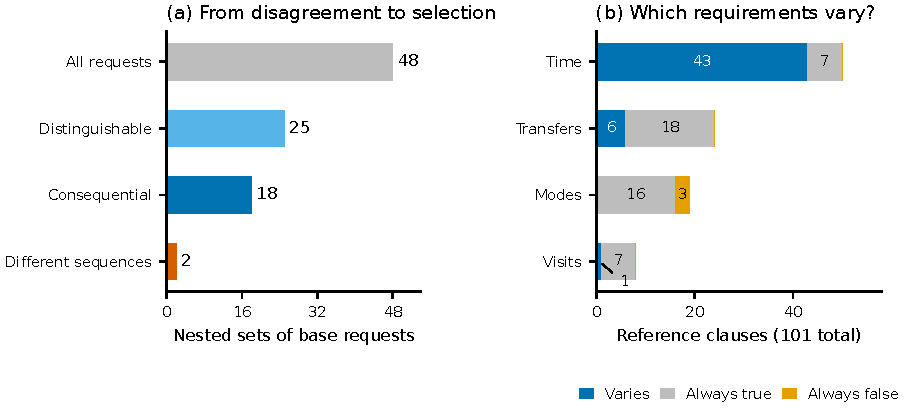
\includegraphics[width=\textwidth]{figures/selector-opportunity.pdf}
\caption{Study 1 connects 48 requests to two divergent sequences through distinguishable and consequential bundles. Uniform weights and tie-breaking explain identical choices. The clause-testing panel shows variation among 101 clauses; no visit clause tests order beyond stop presence. }
\label{fig:opportunity}
\end{figure*}

Both selectors resolve 31/48 requests at budget zero and 33/48 at budgets 1, 2, and 4: three recoveries and one deterioration, a net 4.17-point gain. In the deteriorated case, a correct negative judgment removes a wrong formalization whose initial plan was valid, exposing a dependency between candidate coverage and preservation of a successful decision.
Each selector returns 30/40 valid feasible plans, five invalid plans, and five false infeasibility conclusions. It identifies 3/8 infeasible requests; five give invalid interpretation outputs. No unresolved or infrastructure failures occur. Budget two adds four judgments per method but changes no plan; budget four adds no judgments. Oracle-witness replay reaches 35/48 for both selectors, identifying a shared opportunity in validation rather than an advantage of weighting.
Clause checks identify which requirements the benchmark exercises. Of 101 reference clauses, 50 vary, 48 are always satisfied, and three always violated. Six of 24 transfer clauses vary although 45/48 pools offer zero and one transfer journeys; the two ride bound makes an at most one transfer clause vacuous. All 19 mode clauses are constant, and visits never distinguish ordering beyond stop presence. Removing enumeration caps increases memberships to 77,871 without adding candidate classes or witness partitions for the saved bundles. 



\subsection{Separating Acquisition from Final Choice}

In Study 2, diversified sampling reaches 31/32 candidate coverage compared with 27/32 for independent sampling, while both produce 28/32 correct final outcomes. Figure~\ref{fig:cost} separates acquisition and decision trajectories against consumed tokens. All arms begin at 25/32 coverage and correctness; solver-guided sampling stays there through eight attempts, adding no matching behavior after the shared samples. Mean distinct signatures are 1.41, 1.59, and 1.19 for independent, diversified, and solver-guided sampling. 

\begin{figure*}[t]
\centering
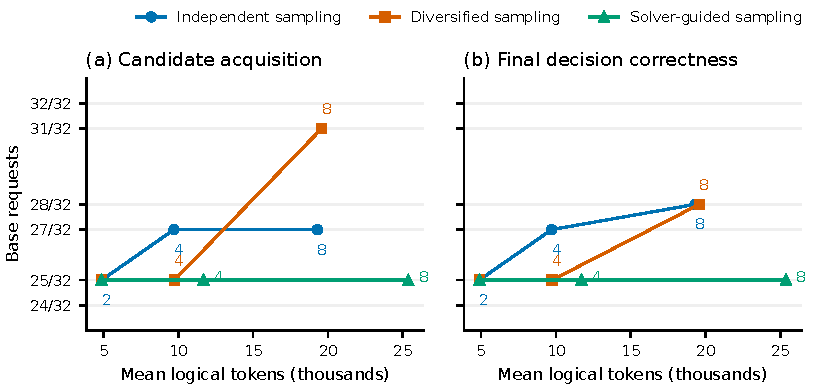
\includegraphics[width=\textwidth]{figures/cost-outcomes.pdf}
\caption{Study 2 separates candidate coverage from final correctness over 32 requests. Labels mark 2, 4, and 8 attempt checkpoints; lines connect only observations. Cost is mean logical input plus output tokens for generation and prefix validation. Diversification increases coverage without changing aggregate final accuracy. Initial samples are shared; allowances remain unexhausted. }
\label{fig:cost}
\end{figure*}

Request level pairing reveals a further distinction behind equal totals: independent sampling wins on one request, loses on one, and ties on 30 against diversified sampling. Solver guided sampling has zero wins, three losses, and 29 ties against each baseline, with different losing sets. Its correctness difference is $-9.38$ percentage points in each comparison. A 10,000 draw base-request bootstrap gives a descriptive 95\% interval of $[-21.88,0]$ points; independent minus diversified gives $[-9.38,9.38]$. 
The baselines return 24/28 valid feasible plans; solver-guided sampling returns 21/28. All identify four infeasible requests correctly; remaining outputs are invalid plans. No final output is unresolved, malformed, or an infrastructure failure; two malformed candidate attempts remain charged. Solver-guided sampling misses the continuation thresholds fixed before fresh outputs on 13 September 2026: at least ten percentage points more candidate coverage and five points more correctness than each baseline.



\subsection{Locating Candidate-to-Decision Transitions}

\begin{figure}[t]
\centering
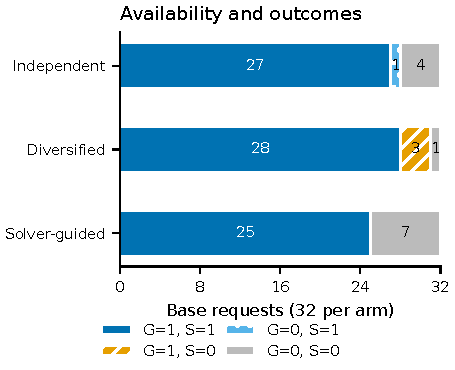
\includegraphics[width=\columnwidth]{figures/joint-outcomes.pdf}
\caption{At 8 attempts, each Study 2 arm contains 32 requests. $G$ denotes candidate coverage and $S$ final correctness. The off diagonal cells identify three diversified sampling selection losses and one independent sampling success without a matching formalization. References remain provisional.}
\label{fig:joint}
\end{figure}

Figure~\ref{fig:joint} shows how candidate coverage relates to final outcomes. In $(1,1),(1,0),(0,1),(0,0)$ order the final counts are $(27,0,1,4)$ for independent, $(28,3,0,1)$ for diversified, and $(25,0,0,7)$ for solver-guided sampling. At four attempts, diversification has $(24,1,1,6)$ as equal marginal coverage and correctness of 25 conceal both off-diagonal outcomes. 
Relative to the provisional references, trace inspection identifies incorrect judgments eliminating the match in all three diversified final $(1,0)$ cases, 2 false positives and one false negative. A fourth loss appears at four attempts. Each final case ends with one class, so an unresolved tie or unused validation opportunity is not the immediate cause. Reference labels recover all three. Across selected witnesses, 11/19 distinct Study 2 judgments and 7/31 Study 1 judgments disagree with provisional references. These disagreements were not independently adjudicated and are not general judge accuracy estimates. 

\begin{figure*}[t]
\centering
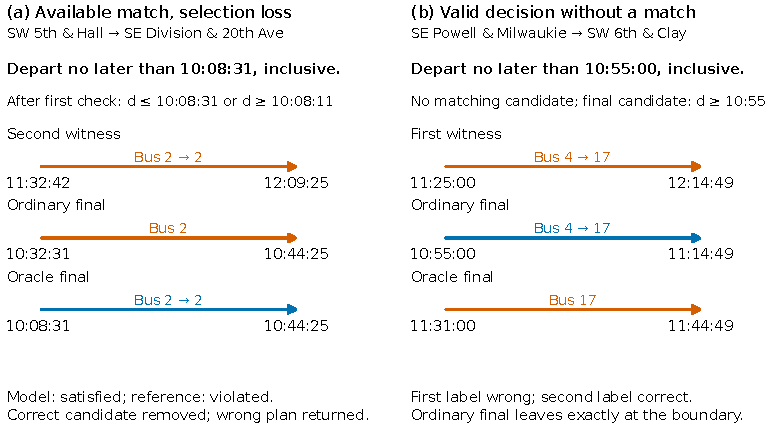
\includegraphics[width=\textwidth]{figures/worked-transit.pdf}
\caption{Separating interpretation from decision correctness in Study 2. The first diversified $(G=1,S=0)$ case at eight attempts (left) shows a false positive discarding the matching upper bound. The sole independent $(G=0,S=1)$ case there (right) shows a lower-bound formalization producing a departure exactly at the requested upper bound; reference-label first witness rejection takes another path. Times are scheduled local service times on 14 September 2026; arrows mark endpoints, not a scaled time axis. Correctness uses provisional references.}
\label{fig:worked}
\end{figure*}

The left example requests departure by 10:08:31. A correct first judgment leaves the matching upper bound and a wrong lower bound. Accepting a second witness departing at 11:32:42 removes the match and yields a 10:32:31 plan. Reference-label replay returns a valid 10:08:31 departure. 

\subsection{Distinguishing Oracle Measurements}

Oracle witness replay substitutes reference labels while retaining bounded elimination and the first surviving candidate. Correctness is 27/32, 31/32, and 25/32: equal to coverage totals here, but measuring a different procedure.
Figure~\ref{fig:worked} (right) explains independent sampling's 28 ordinary versus 27 oracle witness successes. The request requires departure by 10:55; no candidate matches throughout the pool. A wrong positive on an 11:25 departure removes one candidate. A correct second positive retains a lower-bound candidate, whose optimal plan leaves exactly at 10:55 and satisfies the request. Reference-label first witness rejection instead retains a candidate producing an 11:31 departure. Thus reference labels can change the elimination path and lose a valid decision: this procedure is not an accuracy ceiling.
A separate diagnostic asks whether \emph{any existing candidate's deterministically selected output} is correct: 28/32, 31/32, and 25/32 at eight attempts. This restricted best of candidate outputs measure is neither an ordinary selector nor an unrestricted planning bound. 

\subsection{Relating Inference Cost to Discovery}

Final prefix logical input/output tokens total 617,643, 626,497, and 811,760 for independent, diversified, and solver-guided sampling across 32 requests each. Solver guided overhead is 31.43\% and 29.57\%, relative to the corresponding baseline's consumed generation plus validation total. Logical calls are 266, 269, and 262. 
Across prefixes, counting generation once per trajectory and each prefix's judgments gives 833 logical calls and 2,081,931 tokens. Exact caching reduces actual fresh compute to 659 calls and 1,743,059 tokens. Sampling used 1,207.31 measured GPU-resident seconds plus 53.37 for development and a conservative 60-second allowance. The selector study used 358 calls and 681.62 seconds plus 30 seconds. Shared outputs retain full per-arm logical charges.



\section{\uppercase{Applying the Framework}}
\label{sec:recommendations}

\noindent For each base request, retain the universe, source requirements, separate references, raw candidates, signatures, plans, witnesses, judgments, updates, and cost. 
Construct informative tasks: check clause variation and conditional relevance before model evaluation. Identify journeys exposing intended distinctions: different orders with the same stops, transfers around a limit, or departures around a boundary. Pool size alone cannot certify clause testing across experiments. Contrast based inclusion rules improve informativeness without selecting cases for a preferred method.
Target components using evidence: conditional on the references, diversification's increased coverage and three traced losses motivate investigating validation before adding candidates. Conversely, check candidate selected plans in $(0,0)$ cases before attributing failure to missing alternatives.
The $(0,1)$ cell preserves a correct plan's value without certifying its formalization. Precise oracle interventions clarify the remaining opportunity: reference-label replay tests an altered validation path, whereas best-of-candidate outputs measures available decisions.
Connect cost to observable change: report tokens, logical charges, caching, and stopping reasons alongside attempt budgets. Shared time normalization remains a useful engineering baseline. Freeze resource rules and assess component changes on fresh data.
Applying the framework has not itself been shown to improve accuracy or reduce cost.



\section{\uppercase{Limitations}}
\label{sec:limitations}


\noindent The studies contain 48 and 32 bases, one model, and one replicate. Constructed wording, overlapping services, and a shared translation/judgment model constrain generalization. Selection and normalization differ across studies; accuracies must not be pooled. Bootstrap intervals exclude annotation uncertainty, route dependence, and variation over models and prompts.
Separate reference code reduces implementation dependence; developer checks do not establish independent annotation validity. Systematic wording errors could affect $G$ and $S$ together. No clear correction was found in the selector audit. The 80-request worksheet has no completed human-review decisions; disputed judgments remain unadjudicated.
The universe is not the full network. Conditional infeasibility is weaker than real-world impossibility. The subset excludes available non-bus services; transfer clauses can be vacuous, visit clauses do not independently test order, and daytime requests do not test midnight or daylight saving. Study 2's stronger clause checks improve informativeness without broadening these claims.
Matching signatures can conceal semantic differences lacking counterexamples. Clause level signatures expose variation masked by a rejecting conjunct, but source clause associations are not always available. This framework therefore measures bounded behavior, not unrestricted source fidelity; selected witness disagreements are not general judge error rates.
A stronger or independently trained judge, different prompts, or broader coverage could change the comparisons. Repeated lower-bound readings do not establish feedback anchoring. This position developed through exploratory studies, not as a preregistered reporting hypothesis. Its demonstrated value is the diagnostic information obtained here; applicability across models and domains remains open.



\section{\uppercase{Conclusion}}
\label{sec:conclusion}

\noindent We propose a framework linking tested constraints, available interpretations, validation behavior, decisions, and cost. The transit studies demonstrate its explanatory value: opportunity analysis characterizes when selectors can act differently, and joint outcomes separate candidate acquisition from decision selection. The reproducible procedure makes these distinctions available to other planning evaluations. Independent review of references and disputed judgments is needed first. Future studies should measure both available interpretations and selected decisions, stating clause testing and resource use explicitly. 



\subsection*{AI Assistance Disclosure}
\label{sec:ai}
OpenAI Codex \cite{codex} assisted with the code, environment setup and manuscript language editing.


\begin{thebibliography}{99}
\bibitem[Amonkar et~al., 2026]{amonkar}
Amonkar, R., Kayan, C.~E., Lai, Q., Le~Bras, R., and Zhang, L. (2026).
A reality check of language models as formalizers on constraint satisfaction problems.
\emph{arXiv:2505.13252v6}. Preprint; first submitted 2025.
\href{https://arxiv.org/abs/2505.13252v6}{doi:10.48550/arXiv.2505.13252}.

\bibitem[GTFS, 2026]{gtfs}
GTFS (2026). Schedule reference.
\url{https://gtfs.org/documentation/schedule/reference/}. Accessed 13 September 2026.

\bibitem[Mendoza et~al., 2026]{artemis}
Mendoza, D., Mavridou, A., Katis, A., and Trippel, C. (2026).
Automating requirements formalization: Using LLMs and low-complexity distinguishing traces for semantic validation.
In \emph{48th IEEE/ACM International Conference on Software Engineering (ICSE)}.
\href{https://doi.org/10.1145/3744916.3787815}{doi:10.1145/3744916.3787815}.

\bibitem[OpenAI, 2026]{codex}
OpenAI (2026). Codex. AI assistance tool.
\url{https://openai.com/codex/}. Accessed 13 September 2026.

\bibitem[Qwen Team, 2024]{qwen}
Qwen Team (2024). Qwen2.5-7B-Instruct: Official model card.
\url{https://huggingface.co/Qwen/Qwen2.5-7B-Instruct}. Accessed 13 September 2026.

\bibitem[Raza and Milic-Frayling, 2025]{ssv}
Raza, M. and Milic-Frayling, N. (2025).
Instantiation-based formalization of logical reasoning tasks using language models and logical solvers.
In \emph{Proceedings of IJCAI-25}, pages 4633--4641.
\href{https://doi.org/10.24963/ijcai.2025/516}{doi:10.24963/ijcai.2025/516}.

\bibitem[Singh et~al., 2026]{verge}
Singh, V., Cassel, D., Weir, N., Feng, N., and Bayless, S. (2026).
VERGE: Formal refinement and guidance engine for verifiable LLM reasoning.
\emph{arXiv:2601.20055v2}. Preprint.
\href{https://arxiv.org/abs/2601.20055v2}{doi:10.48550/arXiv.2601.20055}.

\bibitem[Tantakoun et~al., 2025]{tantakoun}
Tantakoun, M., Muise, C., and Zhu, X. (2025).
LLMs as planning formalizers: A survey for leveraging large language models to construct automated planning models.
In \emph{Findings of the Association for Computational Linguistics: ACL 2025}, pages 25167--25188.
\href{https://doi.org/10.18653/v1/2025.findings-acl.1291}{doi:10.18653/v1/2025.findings-acl.1291}.

\bibitem[TriMet, 2026]{trimet}
TriMet (2026). GTFS schedule data.
\url{https://developer.trimet.org/GTFS.shtml}. Feed version 20260823-20260910-0900; acquired September 2026.

\bibitem[Wang et~al., 2026]{diversity}
Wang, T., Liu, Z., Chen, Y., Light, J., Liu, W., Chen, H., Zhang, X., and Cheng, W. (2026).
On the effect of sampling diversity in scaling LLM inference.
\emph{arXiv:2502.11027v5}. Preprint; first submitted 2025.
\href{https://arxiv.org/abs/2502.11027v5}{doi:10.48550/arXiv.2502.11027}.
\end{thebibliography}
\end{document}
